\documentclass[review]{elsarticle}
% \usepackage[active, tightpage]{preview}

\usepackage{enumitem}
\usepackage{hyperref}
\usepackage{xcolor}
\hypersetup{
    colorlinks,
    linkcolor={red!50!black},
    citecolor={blue!50!black},
    urlcolor={blue!80!black},
    pdfborder={0 0 0}
}
\usepackage{multirow}
\usepackage{pgfplots}
\usepackage{float}
\usepackage{amssymb}
\usepackage{cleveref}
\usepackage[english]{babel}
\usepackage[utf8]{inputenc}
\usepackage[T1]{fontenc}
% \usepackage{changepage}
\usepackage{longtable}
\usepackage{tabularx}
\usepackage{pdfpages}
\usepackage{incgraph,tikz}
\usepackage[titles]{tocloft}
\setlength{\cftbeforesecskip}{-.5ex}
\renewcommand{\cftsecleader}{\cftdotfill{\cftdotsep}}

% \usepackage[showframe=true]{geometry}
%
\newcommand{\textttt}[1] {\texttt{\footnotesize#1}}
\newcommand{\h} {\hphantom ~ }
% \newcommand{\textttt}[1] {\mbox{\texttt{\footnotesize#1}}}
% \newcommand{\textttt}[1] {
% \begin{verbatim} #1 \end{verbatim}
% }
\pgfplotsset{compat=1.5}
\pgfplotsset
{
	width=0.5\textwidth,
	x tick label style={/pgf/number format/1000 sep=},
  enlarge x limits = 0.0,
  ymajorgrids=true,
	major tick style={draw=none},
  ymin = 0.0,
	every axis/.append style={
		every x tick label/.append style={font=\tiny},
    every y tick label/.append style={font=\tiny},
    every axis label/.append style={font=\small},
    height=37mm,
    width=37mm,
    title style={at={(0.5,0.90)}, font=\normalfont},
    xticklabel style={yshift=4pt}
	}
}

%% `Elsevier LaTeX' style
\bibliographystyle{elsarticle-num}
%
\makeatletter
\def\ps@pprintTitle{%
    \let\@oddhead\@empty
    \let\@evenhead\@empty
    \def\@oddfoot{}%
\let\@evenfoot\@oddfoot}
\makeatother
\begin{document}
%
\begin{frontmatter}
%
\title{Linked Open Social Data for Scientific Benchmarking (Supporting
Information document)}
%
\author[pwr]{Renato Fabbri\corref{corresponding}\fnref{kio-url}}
\ead{fabbri@usp.br}
%
\author[pwr]{Osvaldo Novais de Oliveira Junior\fnref{kio-url}}
\ead{chu@ifsc.usp.br}
%
\cortext[corresponding]{Corresponding author}
\address[pwr]{S\~ao Carlos Institute of Physics, S\~ao Paulo
University, Brazil}
%
\fntext[kio-url]{\textit{URL:} \url{http://www.ifsc.usp.br/}}
%
\begin{abstract}
This is a Supporting Information document which exposes ontological
diagrams and auxiliary tables for the Linked Open Social Data (LOSD)
database. The main document of the article is in~\cite{losd}.
\end{abstract}
%
\begin{keyword}
Big Data, Data Mining, Benchmark Data, Facebook, Twitter, IRC, Email,
Complex Networks, Text Mining
%Hierarchy of Clusters \sep HoC \sep Benchmark Dataset \sep Benchmark Data Generator \sep Artificial Data \sep Cluster Analysis \sep Tree Structured Stick Breaking Process \sep TSSB \sep ...
\end{keyword}

\end{frontmatter}
% \pdfpageheight 8in
\tableofcontents
\section{General guidance}
% \paperheight = 200pt
In this document we provide diagrams
for the provenances in the LOSD:
Facebook, Twitter, IRC, Email, ParticipaBR, Cidade Democrática and AA.
Each provenance diagram was broken in two, one presents the relations
among main classes (blue nodes) and data types (orange nodes), the other presents metadata on the
snapshot.
Every class instance is related to the snapshot instance
by the triple \textttt{class\_uri po:snapshot snapshot\_uri}.
Such triples are omitted for simplicity.
Due to the large number of relations, the rendering of diagrams are
automatized and displays some overlaps.
Even so, the images are useful for grasping what is in current LOSD
and for conducting explorations.
Edges in the diagrams have:
\begin{itemize}
    \item green color if representing an OWL existential
class restriction (all individuals from the class present at least one triple with
the property as predicate);
    \item inverted nip if representing an OWL universal class
        restriction (all individuals presenting triples with the
        property as predicate are from the class);
    \item full edges (non-dashed) if representing a functional property
        axiom (there is at most one triple with the property as the
        predicate for each individual).
\end{itemize}

% \textheight = 100pt
% \pdfpageheight 300pt
Furthermore, this document ends with two sets of tables, one with counts of
triples, participants, edges/interactions/relations and characters,
the other with references for snapshot groups, such as wikipedia or
contact links.


\section{Facebook data}
Each Facebook snapshot is yield by either an user, from which the
friends constitute a friendship network, or a group, which participants
can yield friendship and interaction networks and posts information with
text and some metadata.
Further information is found on the following diagrams, the tables on
the end of this document or in the main document of this
article~\cite{losd}.

% 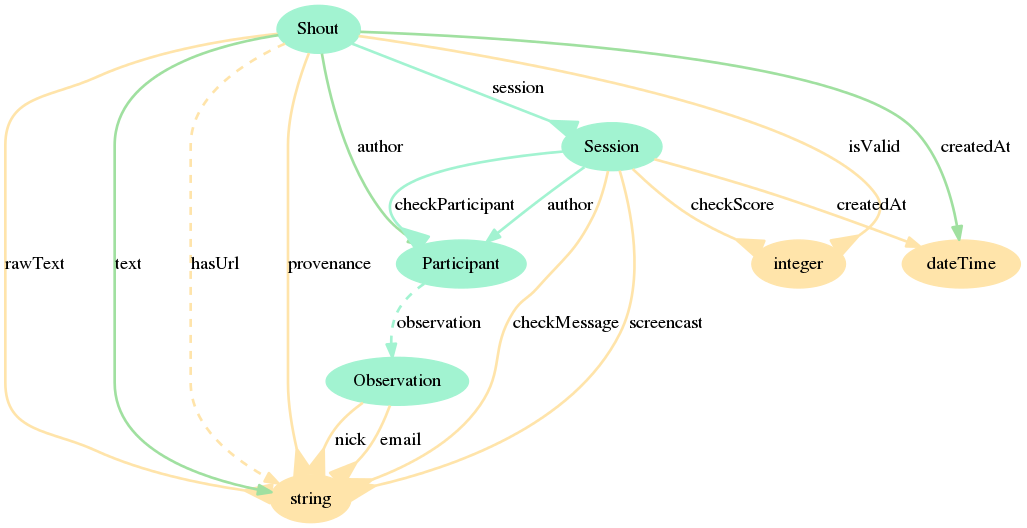
\includepdf{ontologies/aairc.ttl/draw.pdf}
\incgraph[
  overlay={\node[red,below right] at (page.north west) {\Huge Facebook};}
    paper=graphics
][scale=.6]{ontologies/facebook-legacy-Auricultura10042013Friendship.ttl/draw.png}

\incgraph[
  overlay={\node[red,below right] at (page.north west) {\Huge Facebook};}
    paper=graphics
][scale=.5]{ontologies/facebook-legacy-Auricultura10042013Meta.ttl/draw.png}

\section{Twitter data}
Each Twitter snapshot is yield by a hashtag.
Retweets (\textttt{po:retweetOf} are usually considered to yield the interactions between users.
Users are identified through authors \textttt{po:numericID} (global as given by Twitter API)
or \textttt{}.
The database present also \textttt{po:replyTo} and \textttt{po:userMention}
which might also be useful in understanding the networking.
Further information is found on the following diagrams, the tables on
the end of this document or in the main document of this
article~\cite{losd}.

\pdfpageheight 4in
\incgraph[
  overlay={\node[red,below right] at (page.north west) {\Huge
  Twitter };}
    paper=graphics
][scale=.5]{ontologies/twitter-legacy-arenaNETmundialTweet00000.ttl/draw.png}

\incgraph[
  overlay={\node[red,below right] at (page.north west) {\Huge Twitter};}
    paper=graphics
][scale=.7]{ontologies/twitter-legacy-arenaNETmundialMeta.ttl/draw.png}

\section{IRC data}
Each IRC snapshot is yield by an IRC channel.
IRC messages are either server messages (e.g. join and exit channel)
marked with \textttt{po:systemMessage true} and having an \textttt{po:impliedUser user\_uri},
or user messages, which yield interactions through \textttt{po:directedTo} and \textttt{po:mentions} properties.
Text messages without the user names are delivered through the \textttt{po:cleanText} property.
Further information is found on the following diagrams, the tables on
the end of this document or in the main document of this
article~\cite{losd}.
\incgraph[
  overlay={\node[red,below right] at (page.north west) {\Huge IRC};}
    paper=graphics
][scale=.7]{ontologies/irc-legacy-hackerspace-cpsLog00000.ttl/draw.png}
\incgraph[
  overlay={\node[red,below right] at (page.north west) {\Huge IRC};}
    paper=graphics
][scale=.6]{ontologies/irc-legacy-hackerspace-cpsMeta.ttl/draw.png}

\section{Email data}
Each IRC snapshot is yield by an Email list.
Interactions might be considered through \textttt{po:replyTo} relations
Further information is found on the following diagrams, the tables on
the end of this document or in the main document of this
article~\cite{losd}.
\incgraph[
  overlay={\node[red,below right] at (page.north west) {\Huge Email};}
    paper=graphics
][scale=.4]{ontologies/gmane-legacy-.linux.audio.devel1-20000Email00000.ttl/draw.png}
\incgraph[
  overlay={\node[red,below right] at (page.north west) {\Huge Email};}
    paper=graphics
][scale=.5]{ontologies/gmane-legacy-linux.audio.devel1-20000Meta.ttl/draw.png}

\section{ParticipaBR data}
\incgraph[
  overlay={\node[red,below right] at (page.north west) {\Huge
  ParticipaBR};}
    paper=graphics
][scale=.5]{ontologies/participabr.ttl/draw.png}
\incgraph[
  overlay={\node[red,below right] at (page.north west) {\Huge
  ParticipaBR};}
    paper=graphics
][scale=.7]{ontologies/participabr.ttl/draw_circo.png}
\incgraph[
  overlay={\node[red,below right] at (page.north west) {\Huge
  ParticipaBR};}
    paper=graphics
][scale=.7]{ontologies/participabrMeta.ttl/draw.png}

\section{Cidade Democrática data}
\incgraph[
  overlay={\node[red,below right] at (page.north west) {\Huge Cidade
  Democrática};}
    paper=graphics
][scale=.4]{ontologies/cidadedemocratica00000.ttl/draw.png}
\incgraph[
  overlay={\node[red,below right] at (page.north west) {\Huge Cidade
  Democrática};}
    paper=graphics
][scale=.4]{ontologies/cidadedemocratica00000.ttl/draw_circo.png}

\incgraph[
  overlay={\node[red,below right] at (page.north west) {\Huge Cidade
  Democrática};}
    paper=graphics
][scale=.7]{ontologies/cidadedemocraticaMeta.ttl/draw.png}
\section{AA data}
\incgraph[
  overlay={\node[red,below right] at (page.north west) {\Huge AA};}
    paper=graphics
][scale=.6]{ontologies/aairc.ttl/draw.png}
\incgraph[
  overlay={\node[red,below right] at (page.north west) {\Huge AA};}
    paper=graphics
][scale=.7]{ontologies/aaircMeta.ttl/draw.png}

\section{Snapshot references}
\label{sreferences}
\pdfpageheight 10in
\section{Elementary counting in snapshots}

\section*{References}
%
\bibliography{paper}
%\bibliography{myLastBibfile.bib}
%
\end{document} 
